\begin{frame}{Tracking: The Three Main Areas}
  \begin{columns}[t]
    \begin{column}{0.6\textwidth}
      \begin{figure}
        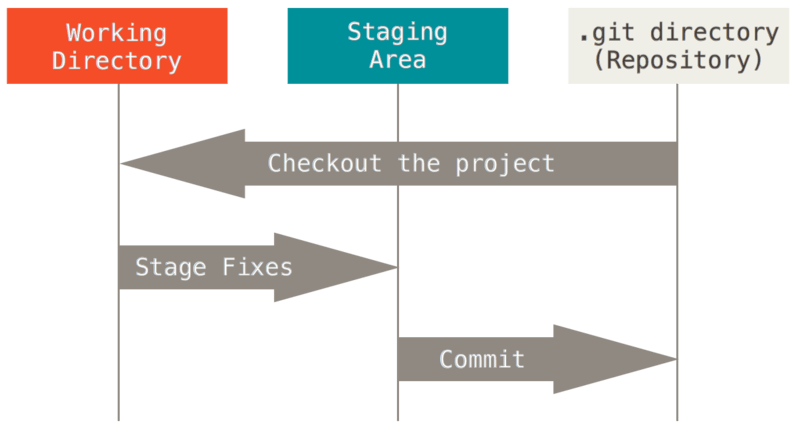
\includegraphics[width=\textwidth]{tracking/areas}
        \caption{The three main areas}
      \end{figure}
      \begin{flushleft}
        Corresponds to the three file stages: Modified, Staged, and Committed.
      \end{flushleft}
    \end{column}
    \begin{column}{0.4\textwidth}
      Working Directory (Tree)
      \begin{flushleft}
        \footnotesize
        A single checkout of one version of the project.
      \end{flushleft}
      Staging Area
      \begin{flushleft}
        \footnotesize
        Stores information about what will go into your next commit.
      \end{flushleft}
      Git directory
      \begin{flushleft}
        \footnotesize
        Stores the version database for your project.
      \end{flushleft}
    \end{column}
  \end{columns}
\end{frame}
